% Sources: docs/datasheet.md, docs/datasheet_pilot_stats.md (generated), docs/protocol.md,
% reports/pilot*/validation.json, paper/figures/fig1.json (generated by scripts/paper_figure.py).
\section{Benchmark}
\label{sec:benchmark}

\begin{figure*}[t]
\centering
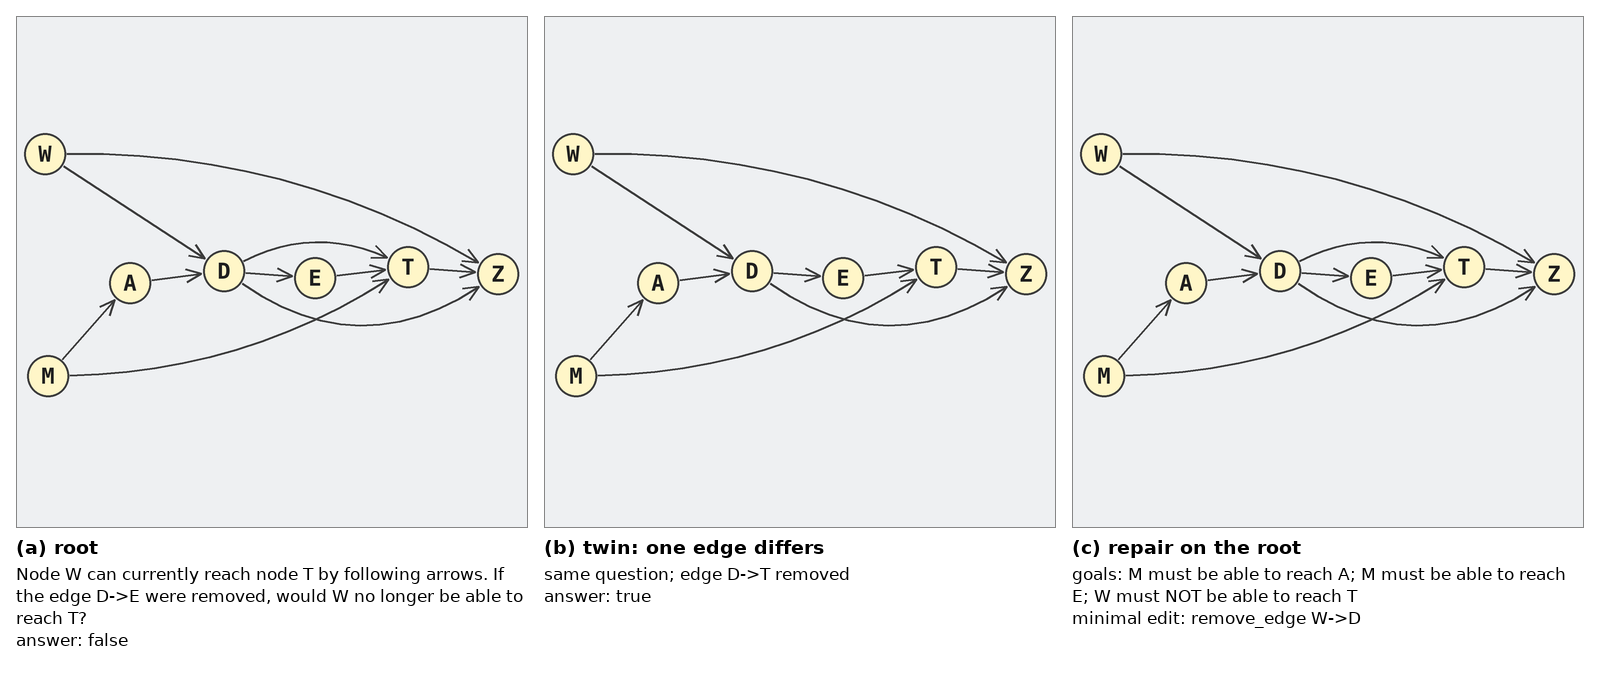
\includegraphics[width=\textwidth]{figures/fig1.png}
\caption{One root graph from the pilot dev split (group \texttt{gabe1987fbac2}).
(a) Critical-edge question; removing $D\!\to\!E$ leaves the path $W\!\to\!D\!\to\!T$, so the
answer is \emph{false}. (b) The answer-flipping twin: the same text with edge $D\!\to\!T$
absent; now the answer is \emph{true}. (c) The repair task on the root image: the only
minimal edit is removing $W\!\to\!D$. Questions, answers and the differing edge are read
from the dataset by \texttt{scripts/paper\_figure.py} and checked against an independent
reference solver in \texttt{tests/test\_paper\_figure.py}.}
\label{fig:twins}
\end{figure*}

\paragraph{Graphs and drawings.}
Each instance is a $512\times512$ drawing of a weakly connected, simple directed graph
without antiparallel edges. Training and in-distribution graphs come from three families
(\texttt{layered\_dag}, \texttt{tree\_plus}, \texttt{sparse\_random}), are placed by one of
four layouts and drawn in one of three styles. Every drawing passes geometric readability
rules (node spacing, edges clear of other nodes, recorded crossings) and a pixel read-back
against the intended drawing.

\paragraph{Tasks.}
The main tasks are \emph{reachability}, \emph{critical edge} (would removing a given edge
disconnect $s$ from $t$?) and \emph{minimal graph repair}: given reachability goals and a
list of edges that may be added (any present edge may be removed), output at most one edit,
or \texttt{unchanged}, or \texttt{impossible}. The repair verifier applies the answer to the
true graph and accepts every minimal solution. Edge existence, shortest-path length and
full graph extraction are secondary tasks. Answers are single JSON objects scored strictly.

\paragraph{Exact labels.}
Labels come from an exact solver and are re-checked by an independent brute-force reference
(transitive closure by Floyd--Warshall). The validator for the pilot build ran 249{,}139
checks with 0 errors; the locked test build ran 258{,}984 checks with 0 errors.

\paragraph{Answer-flipping twins.}
Every main-task question appears with two images that differ by exactly one edge and have
opposite answers (Fig.~\ref{fig:twins}a,b). A predictor that ignores the image therefore
scores at most $0.50$ on each main task, and the share of twin pairs answered correctly on
\emph{both} images measures whether the model uses the edge at all. About a quarter of root
graphs also receive a relabelled and a restyled copy with the same answer (invariance pairs).

\begin{table}[h]
\centering
% Generated by scripts/modelfree_table.py from reports/*/validation.json; do not edit by hand.
\begin{tabular}{lrccccccc}
\toprule
 & & \multicolumn{2}{c}{reachability} & \multicolumn{2}{c}{critical edge} & \multicolumn{3}{c}{minimal repair} \\
\cmidrule(lr){3-4}\cmidrule(lr){5-6}\cmidrule(lr){7-9}
split & roots & const. & text & const. & text & const. & heur. & text \\
\midrule
pilot train & 512 & 0.500 & 0.500 & 0.500 & 0.500 & 0.250 & 0.2637 & 0.500 \\
pilot dev & 200 & 0.500 & 0.500 & 0.500 & 0.500 & 0.250 & 0.2625 & 0.500 \\
test ID & 200 & 0.500 & 0.500 & 0.500 & 0.500 & 0.250 & 0.2650 & 0.500 \\
test style OOD & 200 & 0.500 & 0.500 & 0.500 & 0.500 & 0.250 & 0.2700 & 0.500 \\
test structure OOD & 200 & 0.500 & 0.500 & 0.500 & 0.500 & 0.250 & 0.2650 & 0.500 \\
test combined OOD & 100 & 0.500 & 0.500 & 0.500 & 0.500 & 0.250 & 0.2500 & 0.500 \\
diagnostic family OOD & 100 & 0.500 & 0.500 & 0.500 & 0.500 & 0.250 & 0.2500 & 0.500 \\
diagnostic size OOD & 100 & 0.500 & 0.500 & 0.500 & 0.500 & 0.250 & 0.2600 & 0.500 \\
\bottomrule
\end{tabular}

\caption{Model-free baselines per split, computed by the validator with the real scorer from labels and
instructions alone (no model is involved). \emph{const.}: the better of the two constant answers
(\emph{true}/\emph{false}; for repair \emph{unchanged}/\emph{impossible}), i.e.\ the majority-class
score. \emph{heur.}: the best of three text heuristics for repair (add the edge the goal names, add the
first listed edge, remove the edge named by the first forbidden pair). \emph{text}: the best accuracy of
any predictor that sees the instruction but not the image. Counted on the root and edited images only.}
\label{tab:modelfree}
\end{table}

\paragraph{Model-free baselines.}
Table~\ref{tab:modelfree} gives the scores reachable without the image on every split, including the
locked ones. Both Boolean main tasks are exactly balanced, so a constant answer scores $0.500$; on repair
a constant status scores $0.250$ and no text heuristic exceeds $0.27$. The text-only ceiling is $0.500$
on all three main tasks in every split. These are properties of the builds, fixed when the data was
generated; they are the floor against which every model score in this paper should be read.

\paragraph{Splits without leakage.}
The split unit is the root graph and everything derived from it; no two graphs in
different groups are isomorphic. The locked test build adds held-out drawing styles,
held-out graph families with larger graphs, and their combination; a second locked build
separates the family shift from the size shift. Test labels are guarded in code and opened
once, for the final evaluation.

\paragraph{Reproducibility.}
The content digest (graphs, labels, instructions) was identical on macOS (Python~3.9 and~3.12)
and Linux (Python~3.13); PNG bytes differ between machines through font
rasterisation, so images are rebuilt from the generator and checked by content.

\begin{table}[h]
\centering
\begin{tabular}{lrrr}
\toprule
build / split & root graphs & images & samples \\
\midrule
pilot train & 512 & 2{,}207 & 5{,}092 \\
pilot dev & 200 & 869 & 2{,}012 \\
locked test (ID, style, structure, combined) & 200/200/200/100 & 3{,}078 & 7{,}006 \\
locked diagnostic (family-only, size-only) & 100/100 & 869 & 1{,}978 \\
\bottomrule
\end{tabular}
\caption{Pilot-scale builds (\texttt{docs/datasheet\_pilot\_stats.md}, \texttt{docs/datasheet.md}).
The main build (planned: about 5{,}000 training roots, 7--12 nodes) was not built (Section~\ref{sec:setup}).}
\end{table}
